\section{Theoretical Background}

\subsection{PWA vs. Native}

A mobile application is a software application designed to run on a mobile device. The two smartphone platforms which hold the majority of the market share today are iOS and Android. 
Currently, three major application development techniques are used: Native, Web-based and Hybrid. \\
Native applications are mobile applications developed to function on a specific platform. If a developer wants to release an application on several platforms, a native application has to be developed separately for each platform. \\
Web-based applications utilise internet servers to store data. This results in very low storage size on the user’s device but only allows for access when an internet connection is available. \\
Hybrid applications are a mix between native and web-based. The idea is to write the majority of the code in a way that it can be compiled to run on several platforms. This is done by using a framework like Apache Cordova, React Native or Xamarin. Hybrid development allows for faster and more economic development than native development but produces applications which feel more native than web-based applications.

\todo[inline]{Inludera en paragraf om React Native här?}

Progressive web applications work similarly as web-based applications, but by storing some data on the user’s device they can be accessed offline. PWAs can also access more hardware and functions than web-based applications. PWAs are typically not downloaded through the platforms own application distribution service, but rather accessed through the web browser of the device. 
Accessing the device hardware through the web browser adds another level of abstraction. This means a PWA is not able to access hardware to the same extent as native applications. 

The functionality of PWAs is significantly better on Android devices than on iOS devices.\todo{Källa behövs} PWAs were originally developed for Google Chrome in 2015, and Safari has not had support for the technology until 2018 . Some functionalities are still, at the time of writing, unavailable on iOS devices.
\newline

\begin{table}[ht]
    \centering
    \begin{tabular}{ |c|c|c|c|c|c| } 
        \hline
        \rowcolor{light-gray}
        Feature & Android & iOS & Feature & Android & iOS\\
        \hline
        Screen orientation \& lock & Yes & No & Bluetooth & Yes & No \\ 
        \hline
        Credentials & Yes & No & Push messages & Yes & No \\ 
        \hline
        Background sync & Yes & No & Local notifications & Yes & No \\ 
        \hline
        Advanced Camera Control & Yes & No & VR and AR & Yes & No \\
        \hline
        Vibration & Yes & No & Recording media & Yes & No\\
        \hline
    \end{tabular}
    \caption{\label{tab:yes-no-features}Selection of functions that work on Android but not on iOS for PWA.}
\end{table}


Some functions still remain unavailable on both platforms. The lack of advanced sensors and contact information are two major limitations to PWA. This inhibits some uses for PWAs. The lack of NFC support, for example, makes contactless payments impossible. Some functions have been experimented with, but have yet to appear as officially available.
\newline

\begin{table}[ht]
    \centering
    \begin{tabular}{ |c|c|c|c|c|c| } 
        \hline
        \rowcolor{light-gray}
        Feature & Android & iOS & Feature & Android & iOS\\
        \hline
        Proximity sensors & No & No & Contacts & No & No \\ 
        \hline
        Geofencing & No & No & NFC & No & No \\ 
        \hline
        Task scheduling & No & No & Ambient light & No & No \\ 
        \hline
    \end{tabular}
    \caption{\label{tab:no-feature}Selection of features that do not work on either iOS or Android for PWA.}
\end{table}

React native has access to more functions than PWAs. The biggest drawback of using React native is the poor performance aspect. Javascript is not optimal for heavy computing, therefore applications heavy in graphics tend to perform poorly when developed as React native or PWA compared to native applications. 
When developing a React native, a frame is first built. Then, for each platform, this frame is built upon to make the application act like a platform-native application. About 95\% of the code is built as cross-platform, and the remaining is platform-specific \cite{Ganguly2018}. This means developing a React native application is more budget-friendly than developing two or more native applications. However, the development of React native applications demands knowledge of the different platforms. This differs from PWA, where knowing Javascript is enough to develop one cross-platform application.

\subsection{Usability testing}
The test subjects are presented with a number of tasks or scenarios. The subject will perform these tasks under the supervision of the moderator. The moderator is there to introduce the applications and to help the subject to proceed if they get stuck. Present at the test is also a recorder, who will take notes on the process. This is useful, since the moderator might be too busy with the test subject to properly record what is happening. 
Test subjects are encouraged to think out loud, presenting the researchers with qualitative data in real-time. This also allows the moderator to ask questions during the test, to further understand how the test subject is reacting to the product. 
The tests are recorded, using a camera angled at the device being tested and/or a camera aimed at the participants’ face. This is done to conserve the qualitative data, allowing for later analysis. \newline

\begin{figure}[ht]
	\centering 
    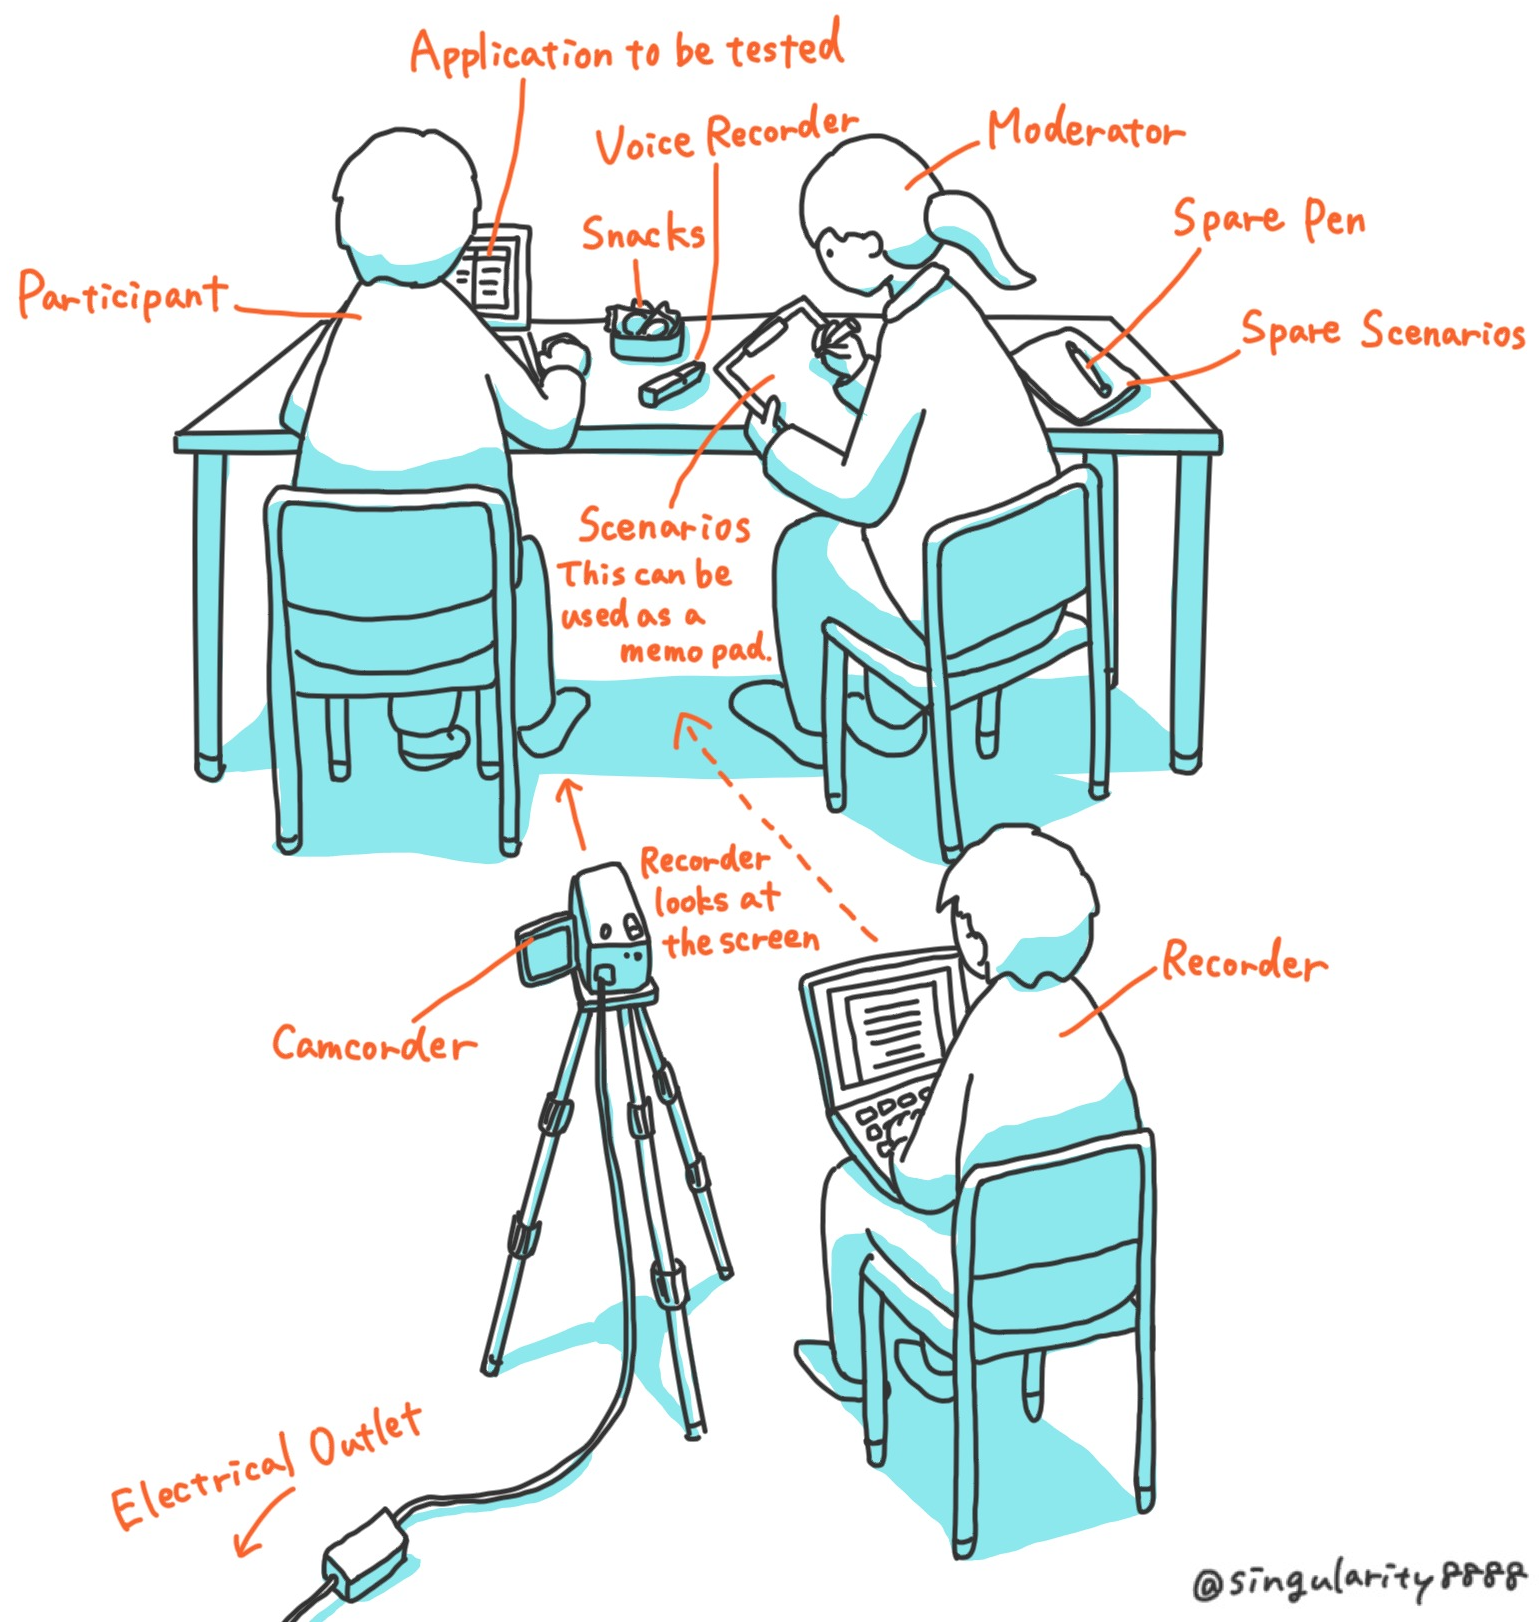
\includegraphics[width=0.8\textwidth]{img/usability_test_example.png}
	\hfill
	\caption{\textit{Diagram of conducting a simple usability test. \cite{Shingyouchi2019} }}
\end{figure}

Quantitative data can be collected as well, often in the form of surveys or questionnaires. The subject will be allowed to assess the products after, or during, the usability tests. 
The system usability scale (SUS) is an easy technique that is reliable even on small sample sizes \cite{SUSUsability}. It uses 10 items that can each be rated on 5 steps from Strongly agree to Strongly disagree. 
\todo[inline]{SUS bilaga här}
Calculating the SUS Score is done by doing the following; for every odd-numbered question, subtract 1 from the score. For every even-numbered question, subtract the score from 5. Sum the scores from even and odd-numbered questions. Then multiply the total with 2.5.
\newline

\begin{table}[ht]
    \centering
    \begin{tabular}{ |c|c|c| } 
        \hline
        \rowcolor{light-gray}
        SUS Score & Grade & Adjective Rating\\
        \hline
        >80.3 & A & Excellent \\ 
        \hline
        68 - 80.3 & B & Good \\ 
        \hline
        68 & C & Okay \\ 
        \hline
        51 - 68 & D & Poor \\
        \hline
        >51 & F & Awful \\
        \hline
    \end{tabular}
    \caption{\label{tab:sus-grading}Grading system for SUS.}
\end{table}

The user experience questionnaire (UEQ) is a fast and reliable way to measure both usability aspects and user experience aspects \cite{UEQOnline}. 
The UEQ can be separated into 6 categories: Attractiveness, Perspicuity, Efficiency, Dependability, Stimulation and Novelty. 
All questions in the questionnaire affect the score of one of these categories. 
If one of the categories is not needed for the test, it’s corresponding questions can be left out of the questionnaire. 

\begin{figure}[ht]
	\centering 
    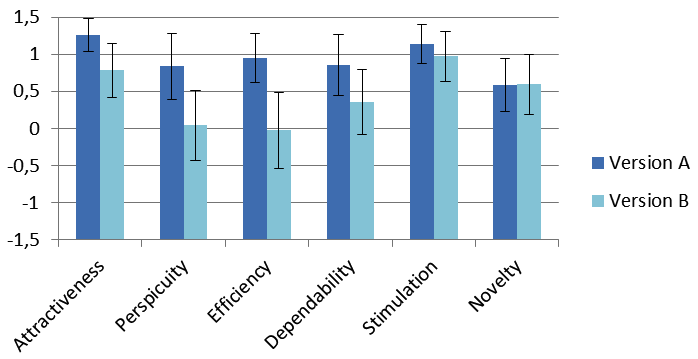
\includegraphics[width=0.9\textwidth]{img/comparative_test_ueq.png}
	\hfill
	\caption{\textit{UEQ result of a comparison between two versions of a product. The mean of each product on each category in blue, the confidence interval marked in black. \cite{SchreppHinderksYhomaschewski2014} }}
\end{figure}

\newpage

\subsubsection{ Comparative usability testing}

During a comparative usability test, test subjects are instructed to use two or more products and compare them. A common practice is to present the subjects with scenarios or tasks, and then let the subjects use the products to complete them. 
Comparative usability testing is conducted to find the usability differences between products. It is a resource-efficient way of testing the usability, as not so many tests are required to find a majority of issues. After just 15 tests, as much as 90\% of problems with the product can normally be found \cite{SixMacefield2016}. 

 \subsection{Multiple-criteria decision making}
 
 MCDM is a collective term for different ways to optimally choose an alternative of something based on multiple, possibly conflicting, criteria. 
 The criteria can be factors such as cost, convenience, quality etc. In most decisions, the criteria have varying importance. 
 This is represented by giving the criteria different weight, a criterion with high weight is more crucial to the final decision than one with a low weight. 
One MCDM method is the Weighted Sum Method (WSM). With WSM, all criteria are given weight by the decision-maker, and each alternative is given a score on each criterion. Depending on the criterion, the score can be decided through quantifiable measures or by assessing qualitative data. For each alternative available, the weight of every criterion is multiplied by the score. These numbers are summed, producing a WSM-score for each alternative. The alternative with the highest WSM-score is the optimal solution.\\
Imagine the following scenario:\\
Charlie is choosing a car. They have three alternatives to choose between: A Kia Picanto, an Audi A8 and a Rolls Royce Phantom. 
Charlie has the following criteria to take into consideration: Price, Comfort, Performance, Prestige. The weights for each criterion and the score for each alternative is shown in the following matrix:
\newline

\begin{table}[ht]
    \centering
    \begin{tabular}{ |c|c|c|c|c| } 
        \hline
        \rowcolor{light-gray}
        & Price & Comfort & Performance & Prestige\\
        \hline
        Weight & 0.50 & 0.25 & 0.20 & 0.05 \\ 
        \hline
        Kia Picanto & 10 & 3 & 2 & 1 \\ 
        \hline
        Audi A8 & 6 & 6 & 8 & 5 \\ 
        \hline
        Rolls Royce Phantom & 1 & 10 & 10 & 10 \\
        \hline
    \end{tabular}
    \caption{\label{tab:WSM-Example}Weighted sum model matrix example.}
\end{table}

The weights indicate how important the different criteria are to the decision maker. Charlie has set the highest score on the criterion Price, meaning they think that Price is the most important criterion. \\
The score for each criterion shows how well an alternative fulfills a criterion. A higher score indicates that the alternative is more superior in a criterion, for example the Rolls Royce Phantom has a score of 10 on comfort, indicating that it is a very comfortable choice. \\
The formula \ref{fig:WSM-formula} is used to calculate the WSM-score. \textit{a} refers to the alternatives, \textit{n} is the number of criteria, \textit{m} is the number of alternatives and \textit{w} is the score of each alternative on a criterion.

\begin{figure}[ht]
	\centering 
    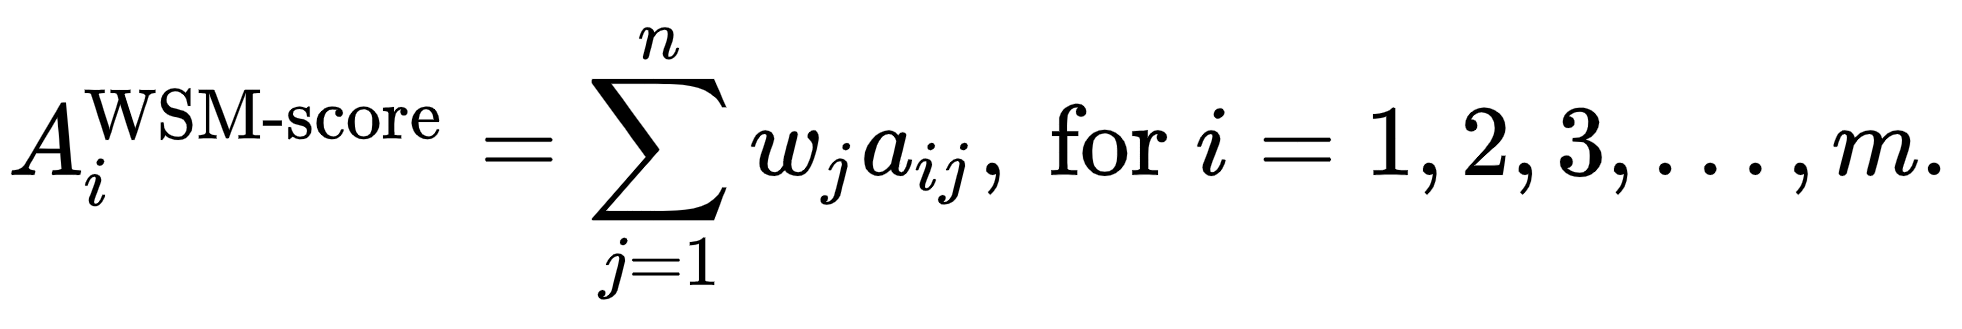
\includegraphics[width=0.8\textwidth]{img/wsm_score_formula.png}
	\hfill
	\caption{\label{fig:WSM-formula}{Formula for calculating WSM score.}}

\end{figure}

\begin{table}[ht]
    \centering
    \begin{tabular}{ |c|c| } 
        \hline
        \rowcolor{light-gray}
        Car model & WSM-score \\
        \hline
        Kia Picanto & 6.2 \\
        \hline
        Audi A8 & 6.35 \\
        \hline
        Rolls royce Phantom & 5.5 \\
        \hline
    \end{tabular}
    \caption{\label{tab:WSM-score}Example WSM score for the example in table \ref{tab:WSM-Example}}
\end{table}

As seen in table \ref{tab:WSM-score}, in this scenario, the most favourable option for Charlie would be the Audi A8, with the Kia Picanto coming in as a close second.

\subsection{Related Work}
